% \setchapterpreamble[u]{\margintoc}
\chapter{What I mean by elimination of reflection}
\labch{elim-reflection-intro}

We presented earlier \acrshort{ETT} and its defining reflection rule.
%
\reminder[-1.0cm]{Reflection rule}{
  \begin{equation*}
    \infer[]
      {\xisterm{\Ga}{e}{\Eq{A}{u}{v}}}
      {\xeqterm{\Ga}{u}{v}{A}}
    %
  \end{equation*}
  See \refdef{reflection}
}
%
The next few chapters are going to be dedicated to its elimination from type
theory: that is how to make a translation from \acrshort{ETT} to type theories
that do not feature reflection.

This work gave rise to a publication~\sidecite[0.2cm]{winterhalter:hal-01849166} that
focused on translating \acrshort{ETT} to \acrshort{ITT}.
However, with Simon Boulier we worked on another version translating directly to
\acrshort{WTT} which I'm going to present here.

\section{Nature of the translation}

\subsection{Syntactical translations are not possible}

First of all we have to wonder about what kind of translation is possible.
We presented earlier~\misref{} the notion of syntactical translation.
Unfortunately it is not possible to devise a syntactical translation to
eliminate reflection from type theory.

Assume we have such a translation given by \(\transl{.}\) and \([.]\) such that
whenever \(\xisterm{\Gamma}{t}{A}\) we have
\(\isterm{\transl{\Gamma}}{[t]}{\transl{A}}\) in the target type theory.
Now let's say we have an inconsistent context in \acrshort{ETT}: \(\Gamma_\bot\)
(one can for instance assume \(0 = 1\) or \(\forall A, A\)), in such a context
anything can have any type because conversion has become trivial.
%
\marginnote[1.4cm]{
  Since \(\Gamma_\bot\) is inconsistent, anything can be proved from it,
  including the equality between the two types \(\mathbb{N}\) and \(\bot\).
  We then use reflection and conversion.
}
\begin{mathpar}
  \infer
    {
      \infer
        {\vdots}
        {\xisterm{\Gamma_\bot}{0}{\mathbb{N}}}
      \\
      \infer
        {
          \infer
            {\vdots}
            {\xisterm{\Gamma_\bot}{\_}{\mathbb{N} = \bot}}
          %
        }
        {\xeqterm{\Gamma_\bot}{\mathbb{N}}{\bot}{\Type}}
    }
    {\xisterm{\Gamma_\bot}{0}{\bot}}
  %
\end{mathpar}
%
It thus follows that in the target you have
\( \isterm{\transl{\Gamma_\bot}}{[0]}{\transl{\bot}} \).
Similarly you would have
\( \isterm{\transl{\Gamma_\bot}}{[0]}{\transl{\mathbb{N}}} \). This means
that both \(\bot\) and \(\mathbb{N}\) should be translated to similar things
(to convertible types in case the target theory has uniqueness of type), without
being able to exploit the knowledge that \(\Gamma_\bot\) is inconsistent
because of the syntactical nature of the translation.

\todo{Make things clearer}
Even worse, translations should preserve falsehood meaning in particular that
the translation of \(0\) should imply a proof of \(\bot\) in the target.
This is not a concrete proof that it is impossible but rather an argument
to see that such a translation would not behave well. One of the reasons is
that it would translate terms, types and contexts independently when it cannot.
Another is that an \acrshort{ETT} term does not contain any hints with respect
to the uses of reflection.

\subsection{Our translation(s)}

If we go back to the notion of proof~\misref, it becomes apparent that
syntactical translations do not work because we would not be translating proofs
but only partial ones; in other words terms in \acrshort{ETT} are not proofs
because they are insufficient to recover a typing derivation\sidenote{Because
type-checking is undecidable.}.
Thus comes the question of what is a \emph{suitable proof} in \acrshort{ETT}.
There is probably an intermediate structure between the term and the full
derivation that fits this role in the form of a term together with explicit
casts, however, in the setting of this thesis, we will still use complete
typing derivations in \acrshort{ETT} as \emph{proofs}.

Many problems stem from this approach unfortunately. Since we're translating
derivations there is no guarantee that the same term \(t\) in
\(\xisterm{\Gamma}{t}{A}\) and \(\xisterm{\Delta}{t}{B}\) will be translated
twice to the same term, this actually goes even for two different derivations
of the same judgement \(\xisterm{\Gamma}{t}{A}\).
This seems like a big obstacle to compositionality and would be iredeemable
without extra care regarding how individual judgements are translated.

We solve these problems by relating translations of a term (respectively
type and context) to the term itself, \emph{syntactically}.

\section{Target(s) of the translation}

Strictly speaking, elimination of reflection should be a translation from a
certain type theory \(T\) extended with reflection to \(T\) itself.
To fit this framework, we would provide a translation from \acrshort{ETT}
to \acrshort{ITT}. With Simon Boulier we discovered however that it is possible
to do something even stronger and go directly to a much weaker theory where
the notion of conversion is removed, \acrshort{WTT}.

\begin{figure}[hb]
  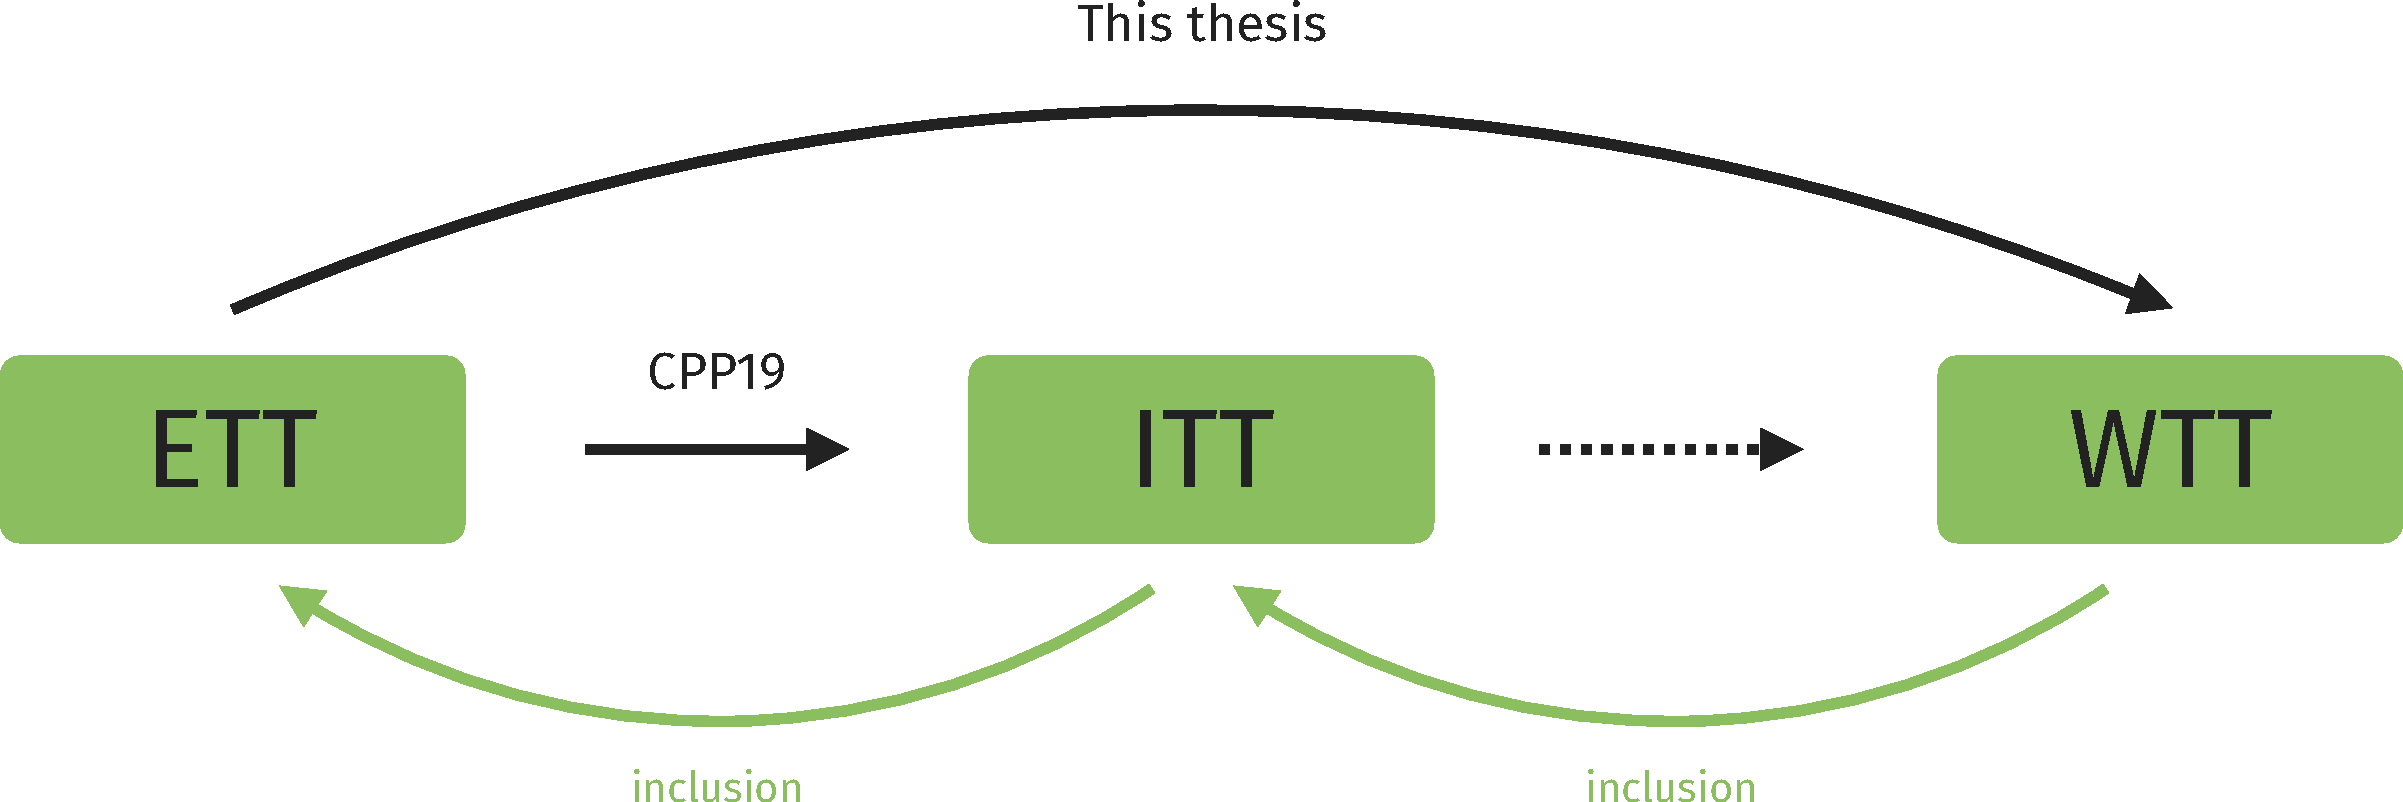
\includegraphics[width=0.9\textwidth]{elim-reflection-summary}
\end{figure}

From a translation of \acrshort{ETT} to \acrshort{WTT} we get an indirect one
from \acrshort{ETT} to \acrshort{ITT} as well as one from \acrshort{ITT} to
\acrshort{WTT}.
\marginnote[-0.5cm]{In both cases we exploit the fact that \acrshort{ETT}
extends \acrshort{ITT} which in turn extends \acrshort{WTT}.}

Note that in both cases, we're not dealing with arbitrary notions of
\acrshort{ITT} and \acrshort{WTT} but ones extended with some principles on
equality that will be described in \vrefsec{ext-principles}.

\section{Goal of the translation}

Why would we want to eliminate reflection? The first interest is that it
justfies that adding the reflection rule preserves consistency.
The main take-away however comes from the fact that we can show that
\acrshort{ETT} is conservative over both \acrshort{ITT} and \acrshort{WTT},
meaning that in order to prove a statement in one of those, it is enough
to prove it using the refleciton rule.
%
\reminder[-2.3cm]{Conservativity (roughly)}{
  A theory \(\mathcal{S}\) is said to be \emph{conservative} over a
  theory \(\mathcal{T}\) when every statement in \(\mathcal{T}\) that
  is provable in \(\mathcal{S}\) is also provable in \(\mathcal{T}\).
}
%

This can have practical use when proving theorems in a proof assistant like \Coq
which doesn't have reflection. If the translation is constructive, it gives
rise to an algorithm to transform a proof using reflection into a proof without.

The deduced \acrshort{ITT} to \acrshort{WTT} even teaches us that computation
is more of a commodity than a necessity as proofs can be transformed not to
exploit any computational behaviour.

\section{Extensionality principles on equality}
\labsec{ext-principles}

As we said earier, the \acrshort{ITT} and \acrshort{WTT} we consider are
actually extended with extensional principles on equality.
The main principles we require are \acrshort{UIP} and fonctional extensionality.
These two principles are valid statements of \acrshort{ITT} and \acrshort{WTT}
which are provable in \acrshort{ETT}, to show \acrshort{ETT} is a conservative
extension of the target, it must be provable in it; as it isn't the case we need
to extend the target with those principles.
\reminder[-3.6cm]{\acrshort{UIP}}{
\[ \Pi\ x \ y\ (e \ e' : x = y).\ e = e' \]
}
\reminder[-2.1cm]{\Acrshort{funext}}{
\[ \Pi\ f \ g .\ (\Pi x.\ f\ x = g\ x) \to f = g \]
}

For \acrshort{UIP} it can be show equivalent to Streicher's axiom K
\[
\begin{array}{rcl}
  \mathtt{K} & : & \Prod{A: s} \Prod{x :A} \Prod{e : x = x} e = \refl{x} \\
\end{array}
\]
where \(s\) is a sort, using the elimination on the identity type.
K is provable in \acrshort{ETT} by considering the type
\[
  \Prod{A: s} \Prod{x \ y:A} \Prod{e : x = y} e = \refl{x} \\
\]
which is well typed (using the reflection rule to show that $e$ has
type $x= x$) and which can be inhabited by elimination of the identity
type.

In the same way, \acrshort{funext} is provable in \acrshort{ETT} as shown by the
following diagram.
\[
\begin{array}{cll}
  &\Prod{x : A} f\ x = g\ x \\
  \to & x : A \vdash f\ x \equiv g\ x &
  \mbox{by reflection} \\
  \to &  (\lambda (x:A). {f \ x}) \equiv (\lambda{(x:A)}.{g \ x}) &
  \mbox{by congruence of $\equiv$} \\
  \to &  f \equiv g & \mbox{by $\eta$-law} \\
  \to &  f = g
\end{array}
\]

Therefore, applying our translation to the proofs of those theorems in
\acrshort{ETT} gives corresponding proofs of the same theorems in the target.

As I said, \acrshort{UIP} is independent from \acrshort{ITT}, as first shown by
Hofmann and Streicher using the groupoid model~\sidecite{groupoid-interp}, which
has recently been extended in the setting of univalent type theory using the
simplicial or cubical models~\sidecite{kapulkin2012simplicial,coquand:cubical}.

Similarly, \acrshort{funext} is independent from \acrshort{ITT}, it is folklore
but has recently been formalised by Boulier \emph{et al.} using a simple
syntactical translation~\sidecite{boulier17:next-syntac-model-type-theor}.

As previously said in \vrefsubsec{wtt}, \acrshort{WTT} has to be extended with
more principles in the vein of functional extensionality, like extensionality
of \(\Pi\)-types for similar reasons.

\section{Basic idea of the translation}

The basic idea behind the translation is to interpret conversion using the
internal notion of equality, \ie the identity type.
The naive approach would thus be to use transport to simulate the conversion
rule.
\reminder[-2.3cm]{Transport}{
Transport turns an equality \(e : A = B\) into a map
\(A \to B\).
}

This means however that for two terms \(a : A\) and \(b : B\) such that
\(A \equiv B\) and \(u \equiv v\) in \acrshort{ETT}, there translations
become comparable in the target only up-to the equality
between the two types. \([u] =_{[A]} [v]\) doesn't necessarilly make sense
anymore.

To solve this proper we use instead a notion of heterogeneous equality.
This is also the approach followed by
Oury~\sidecite[1.7cm]{oury2005extensionality}
although we decided on a slightly different presentations of heterogeneous
equality to avoid the axioms involved with the use of \acrshort{JMeq}.
\reminder[-2.3cm]{Heterogenous equality}{
\(\Heq{T}{t}{U}{u}\), equality between \(t : T\) and \(u : U\) is defined as
\(\Sum{p:\Eq{}{T}{U}} \Eq{}{\transpo{p}\ t}{u}\).
}

During the translation, the same term occurring twice can be
translated in two different manners, if the corresponding typing
derivations are different. Even the types of the two different
translations may be different.
%
However, we have the strong property that any two translations of the
same term only differ in places where transports of proofs of equality have been
injected.

To keep track of this property, we introduce the relation $t \sim t'$
between two terms of the target, of possibly different
types\sidenote{The relation is fully syntactic.}.
%
The crux of the proof of the translation is to guarantee that for
every two terms $t_1$ and $t_2$ such that $\isterm{\Ga}{t_1}{T_1}$,
$\isterm{\Ga}{t_2}{T_2}$ and $t_1 \sim t_2$, there exists $p$ such that
$\isterm{\Ga} {p} {\Heq{{T_1}} {{t_1}} {{T_2}} {{t_2}}}$.

During the proof, variables of different but (propositionally) equal
types are introduced and the context cannot be maintained to be the same
for both $t_1$ and $t_2$. Therefore, the translation needs to keep
track of this duplication of variables, plus a proof that they are
heterogeneously equal.
%
This mechanism is similar to what happens in the (relational) internal
parametricity translation in \acrshort{ITT} introduced by
\sidecite[-0.4cm]{bernardy2012proofs} and recently rephrased in the setting of
\MetaCoq~\sidecite{DBLP:conf/itp/AnandBCST18}. Namely, a context is not
translated as a telescope of variables, but as a telescope of triples
consisting of two variables plus a witness that they are in the
parametric relation: \(x : A\) is (roughly) sent to
\(x_1 : A_1, x_2 : A_2, x_\varepsilon : A_\varepsilon\ x_1\ x_2\).
%
In our setting, this amounts to consider telescope of triples
consisting of two variables plus a witness that they are
heterogeneously equal. We can express this by considering the
following dependent sums:
\[
\Pack{A_1}{A_2} := \Sum{x:A_1} \Sum{y:A_2} \Heq{A_1}{x}{A_2}{y}.
\]

This presentation inspired by the parametricity translation is crucial
in order to get an effective translation, because it is necessary to
keep track of the evolution of contexts when doing the translation on
open terms.
%
This ingredient is missing in Oury's work~\sidecite{oury2005extensionality},
which prevents him from deducing an effective (\ie constructive and
computable) translation from his theorem.
The construction of this relation is discussed in \vrefch{elim-rel}.

\todo{Have a presentation of the common syntax? Or should it be done in the
flavous chapter?}